% Kettleworks — a town that is four chimneys and a decision to stay.
%
% Written by filling in tikz_figure_prompt.md.
\documentclass[tikz,border=4pt]{standalone}
\usetikzlibrary{calc}

% ---- tunables -------------------------------------------------------------
\newcommand{\Unit}{0.055cm}
\newcommand{\Edge}{2.2pt}
\newcommand{\Stacks}{4}        % chimneys
\newcommand{\StackW}{7}
\newcommand{\Ground}{10}

\definecolor{brick}{HTML}{7A4A32}
\definecolor{brickdark}{HTML}{4E2E1E}
\definecolor{smoke}{HTML}{9A9AA6}
\definecolor{ember}{HTML}{C08A2E}
\definecolor{ink}{HTML}{101018}

\begin{document}
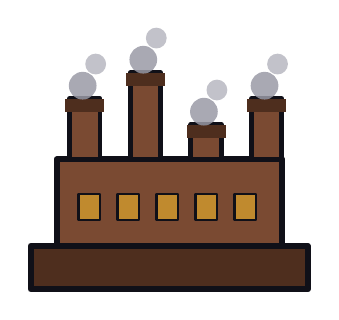
\begin{tikzpicture}[x=\Unit,y=\Unit, line join=round, line cap=round]

  % ---- ground -------------------------------------------------------------
  \fill[brickdark,draw=ink,line width=\Edge] (0,0) rectangle (64,\Ground);

  % ---- the works ----------------------------------------------------------
  \fill[brick,draw=ink,line width=\Edge] (6,\Ground) rectangle (58,30);
  % Windows, lit, because somebody is on shift.
  \foreach \x in {11,20,29,38,47} {
    \fill[ember,draw=ink,line width=1.0pt] (\x,16) rectangle ++(5,6);
  }

  % ---- chimneys, each a little different so it is not wallpaper -----------
  \foreach \i in {1,...,\Stacks} {
    \pgfmathsetmacro\x{9 + (\i-1)*14}
    \pgfmathsetmacro\h{38 + mod(\i,3)*6}
    \fill[brick,draw=ink,line width=1.8pt] (\x,30) rectangle ++(\StackW,\h-30);
    \fill[brickdark] (\x-1,\h-3) rectangle ++(\StackW+2,3);
    % Smoke, leaning the same way off every stack.
    \fill[smoke,opacity=0.85] (\x+3,\h+3) circle (3.2);
    \fill[smoke,opacity=0.6] (\x+6,\h+8) circle (2.4);
  }

  % ---- annotations: none. --------------------------------------------------

\end{tikzpicture}
\end{document}

% ---- self-check ------------------------------------------------------------
% 1. Standalone class, compiles alone with pdflatex.
% 2. Chimney count, width and the ground line are tunables at the top.
% 3. \foreach draws the windows and every chimney with its smoke.
% 4. Order runs ground -> works -> chimneys, so smoke is never behind brick.
% 5. Rectangles and circles only.
